\section{\dis Application Requirements}
\label{sec:requirements}
In this section, we explore the second question: what support do applications in \dis require from the network, in terms of bandwidth and latency, to maintain the performance observed in existing \pdis? We start by describing the methodology used to explore this question (\S\ref{ssec:rmethod}), discuss the requirements (\S\ref{ssec:rr}) and discuss how current technology trends are favorable towards achieving these requirements (\S\ref{ssec:rtt}).

\subsection{Methodology}
\label{ssec:rmethod}
For memory accesses, there are two main sources of performance penalty. First, software overhead for trap and page eviction. Depending on the page eviction algorithm used, existing research prototypes report this per-page overhead to be roughly in the range of $2$--$6\mu$s. However, it is expected that this overhead can be reduced to sub-microseconds with faster CPUs and software optimization, making this overhead insignificant. The second source of performance penalty is the page transfer time over the network. In comparison to the first overhead, the network transfer times could be significant. We, thus, focus on the second overhead, by looking into the performance requirements of the network to support remote memory access, without introducing significant performance penalty.

We use the SIT, described in \S\ref{sec:workloads}, to emulate remote memory access. Specifically, SIT implements a special swap device (backed by physical memory rather than a disk) allowing us to inject artificial delays to emulate network round-trip latency and bandwidth for each paging operation. We measure relative performance on the basis of throughput or request completion time as compared to the zero-delay case. \rc{Talk about the limitations --- does not take into account OS overhead, and end-to-end network delays.}

\subsection{Requirements}
\label{ssec:rr}

%
\begin{figure*}
  \centering
    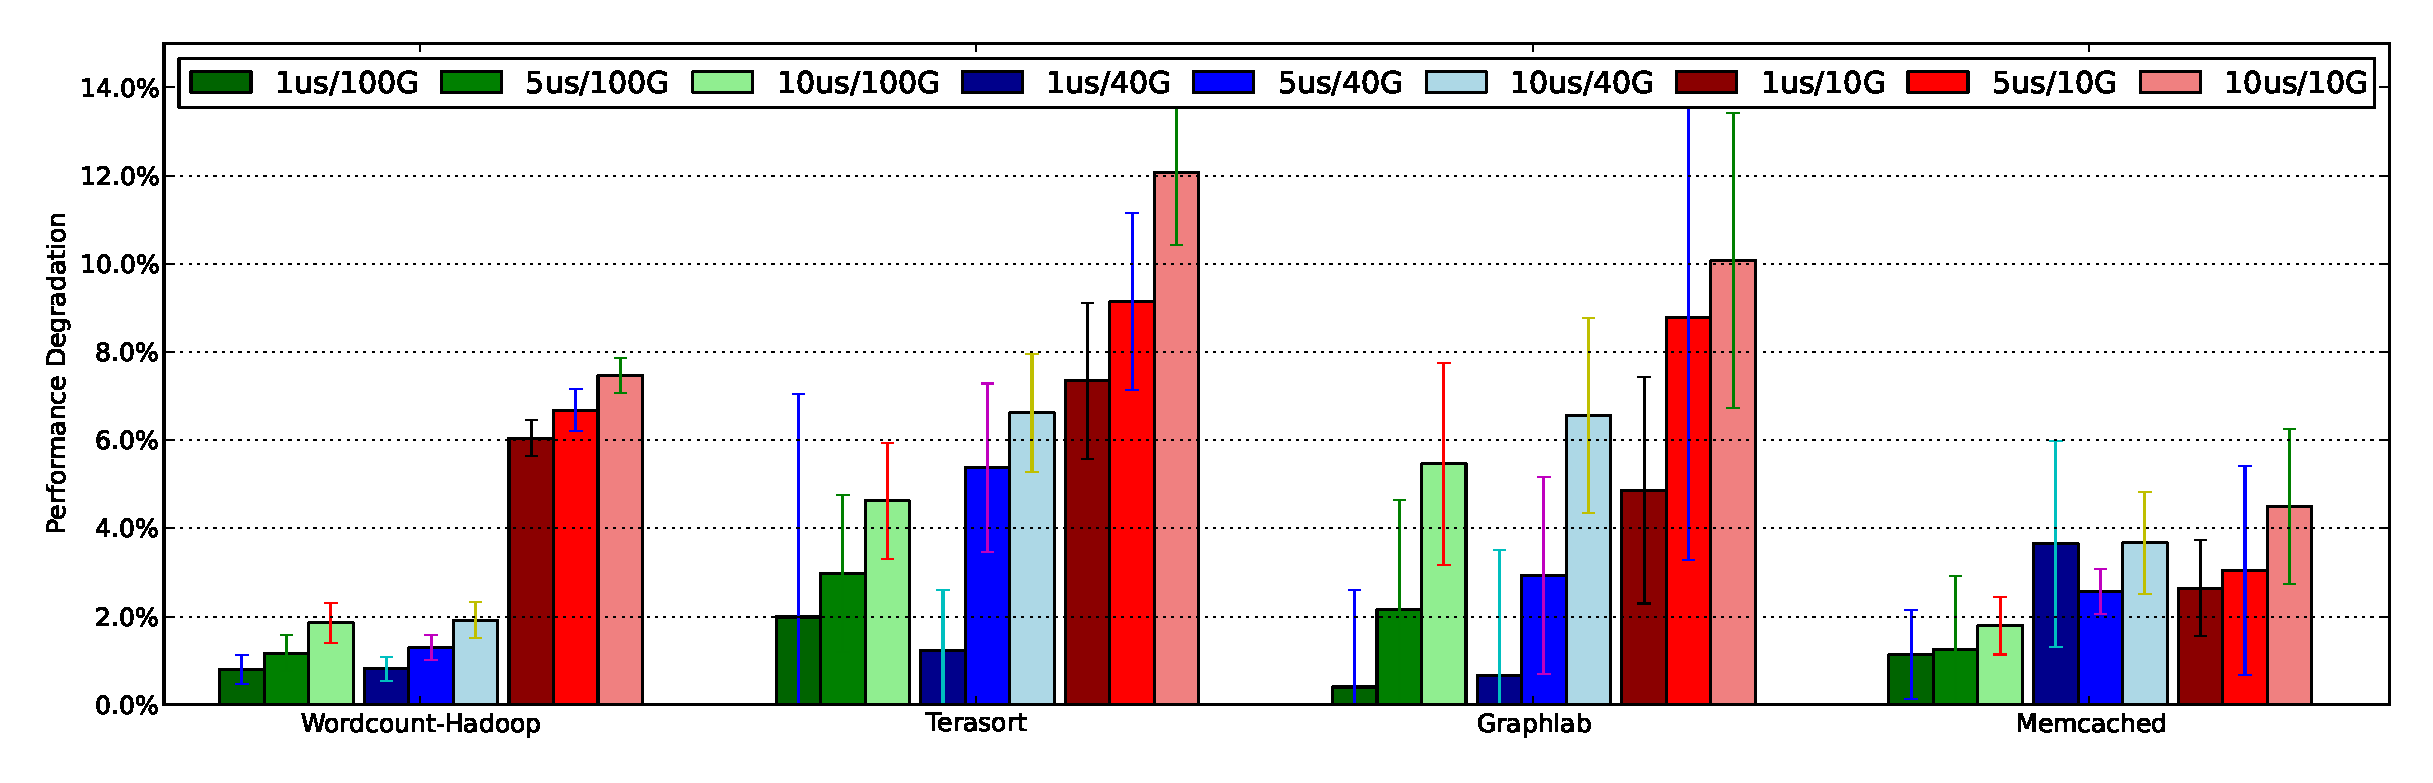
\includegraphics[width = 7in]{img/vary_latency_bw.eps} 
  \caption{\small{\rqc{The main figure for varying latency and bandwidth. One bar graph, one set of bars for each application; one bar for each configuration.}}}
  \label{fig:latb}
\end{figure*}
%
Figure~\ref{fig:latb} shows the application layer performance for six different combinations of network bandwidth and latency configurations. These results, as earlier, were obtained by setting the local cache to be $30\%$ of the working memory of each application. We discuss the results in-depth below. 

\paragraphb{$40$Gbps, $5\mu$s is sufficient}
We start by observing that given a network with $40$Gbps access link bandwidth, and end-to-end delay of $5\mu$s, the application-level performance in \dis can be brought down to within $5\%$ of that in \pdis. While $100$Gbps network bandwidth does not provide significant benefits over the $40$Gbps case, reducing the latency down to $1\mu$s can lead to applications observing essentially no performance degradation. In the hindsight, this is not surprising given our results from \S\ref{sec:workloads}, where we established that the network traffic volume does not increase significantly in \dis compared to \pdis, and that the network flows are dominated by short (latency-sensitive) memory access flows. \rc{$\gets$ needs more concrete intuition; remote memory faster than local disk; applications heavily pipelined; CPU bottleneck?}

\paragraphb{Benefits of remote memory}
First, given sufficient network bandwidth and small network latencies, use of remote memory can drastically improve application performance compared to traditional disk-based swap. Since the working set size is hard to predict in advance, memory tends to be highly over-provisioned in datacenter servers to prevent thrashing. Disaggregated remote memory can reduce this waste by providing an elastic memory capacity pooled at the datacenter scale. 

%
\begin{figure}
  \centering
    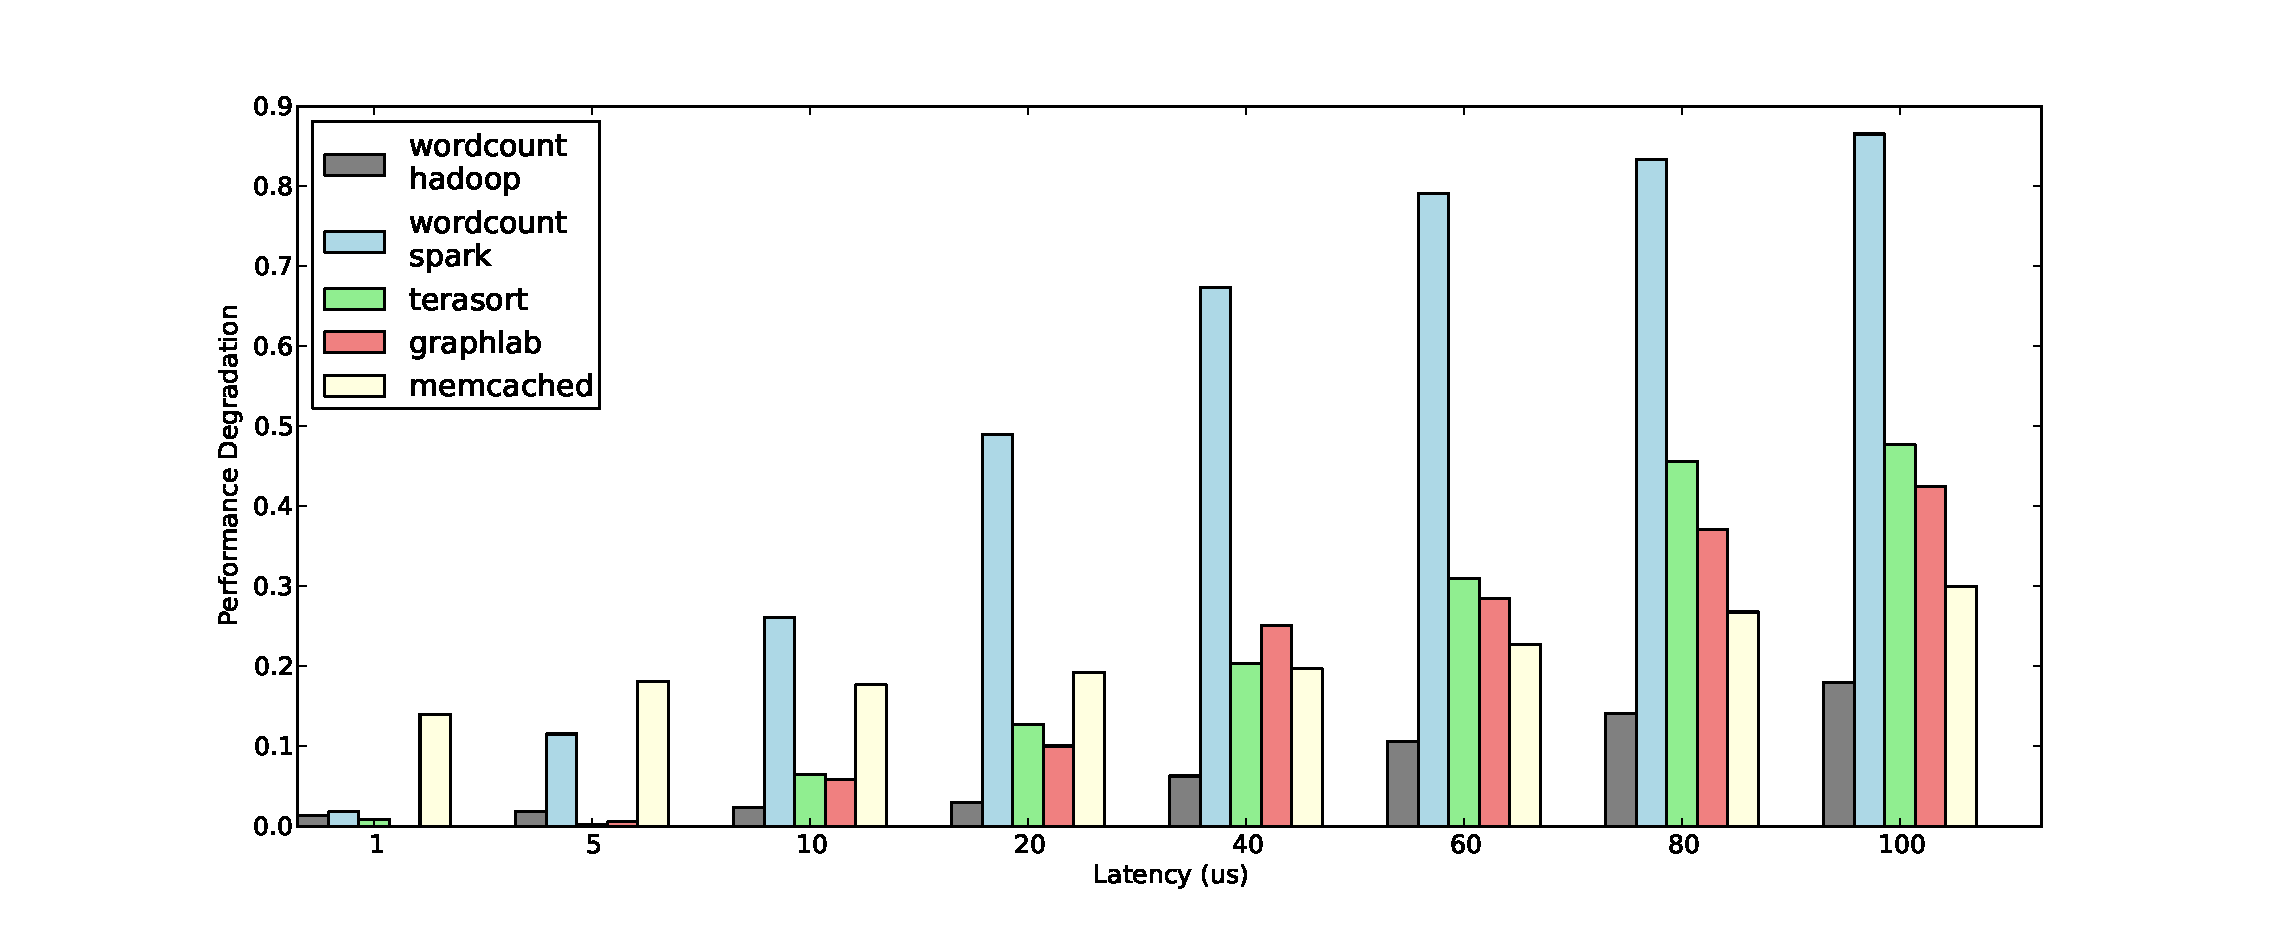
\includegraphics[width = 3.5in]{img/fix_bw_vary_latency.eps} 
  \caption{\small{\rqc{Fix bandwidth to 10Gbps. Vary latency from 1us to some large number. conclude that end-to-end latency has significant impact}}}
  \label{fig:impl}
\end{figure}
%
\paragraphb{Reducing latency more important than increasing bandwidth}
Second, low latency is more important than high bandwidth. The $100$Gbps bandwidth did not provide any significant improvement over the $40$Gbps link. In contrast, $10\mu$s round-trip latency causes noticeable performance degradation, as compared to the $1\mu$s case.

%
\begin{figure}
  \centering
    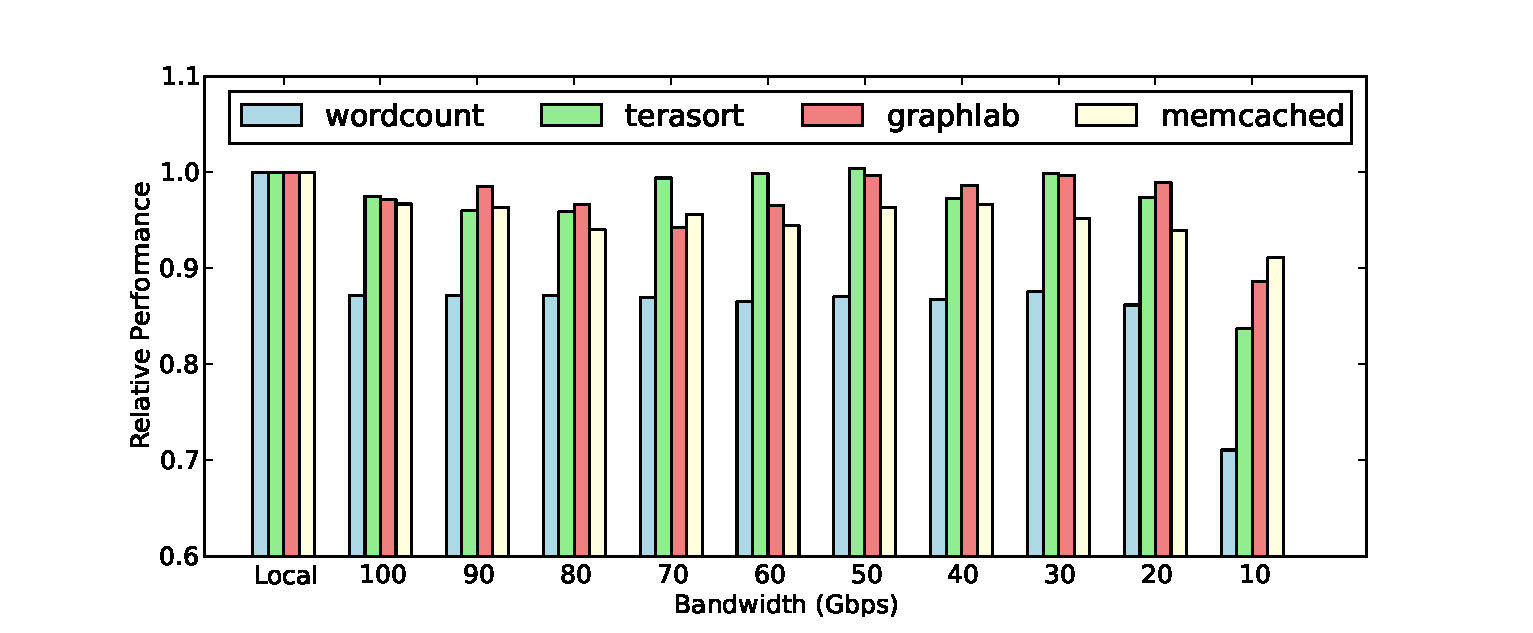
\includegraphics[width = 3.5in]{img/fix_latency_vary_bw.eps} 
  \caption{\small{\rqc{Fix end-to-end latency to 5us. Vary bandwidth from 10Gbps to 100Gbps. conclude that bandwidth does not have any significant impact after 40Gbps.}}}
  \label{fig:impb}
\end{figure}
%


%
\begin{figure}
  \centering
    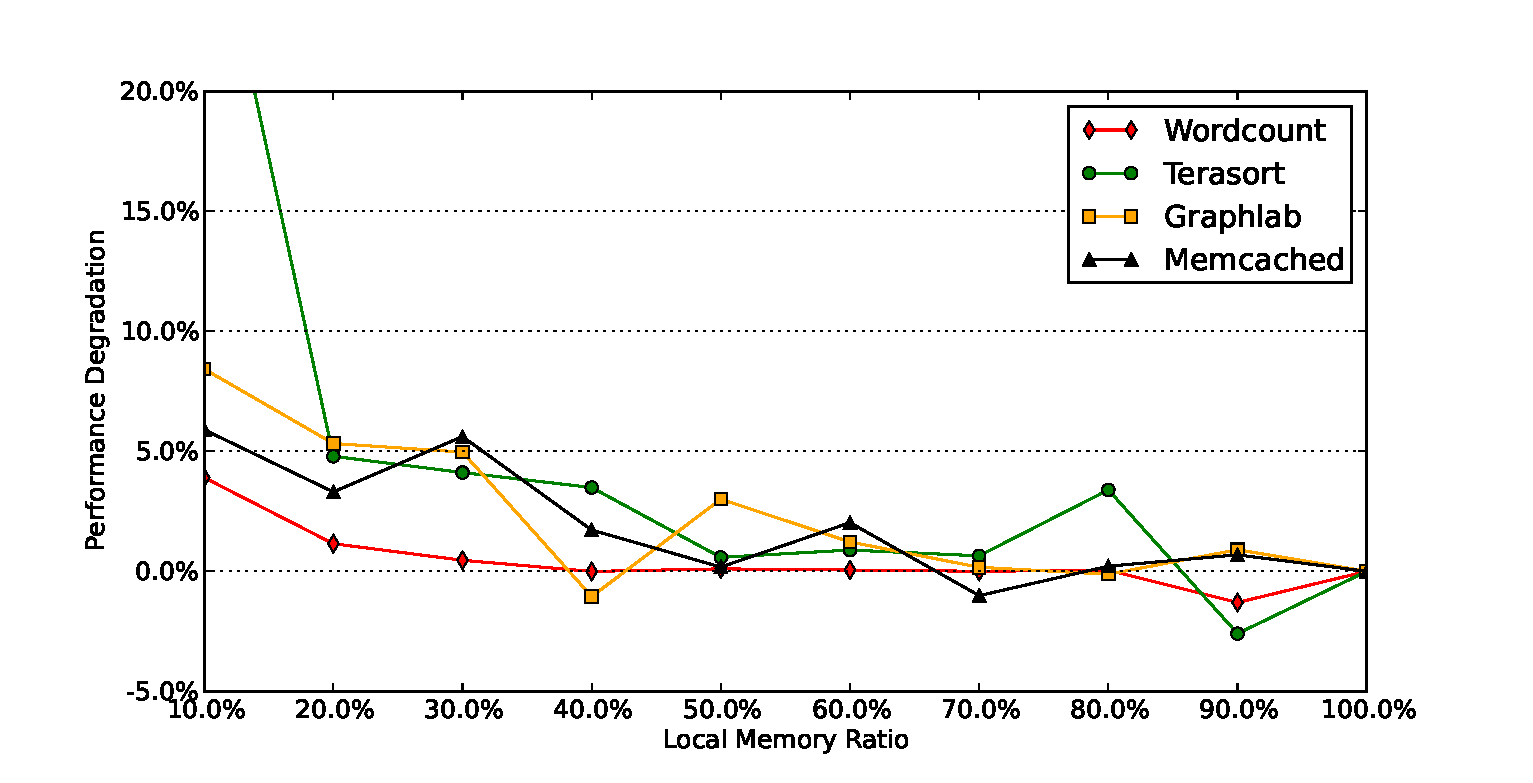
\includegraphics[width = 3.5in]{img/vary_remote_mem.eps} 
  \caption{\small{\rqc{Fix latency at 5us, bandwidth at 40Gbps, Vary local memory from 0\% to 90\% of the total memory of the EC2 instance}}}
  \label{fig:impb}
\end{figure}
%


\subsection{Technology trends}
\label{ssec:rtt}

\begin{itemize}
	\item Implications? Why are current technology trends favorable?
	\item Feasibility: Existing solutions and technology trends
\end{itemize}